\documentclass[a4paper]{article}
\usepackage[fontset=fandol]{ctex}
\usepackage[margin=2cm]{geometry}
\usepackage{pdfpages}
\usepackage{hyperref}
\usepackage{longtable}
\title{Stanford CS224R Deep Reinforcement Learning}
\author{Codex based on course page, slides, subtitles, and lecture videos}
\date{\today}
\begin{document}
\maketitle
\tableofcontents
\newpage
\section*{课程说明}
本讲义先逐讲生成，再按播放列表顺序合并。
\addcontentsline{toc}{section}{课程说明}
\section*{课程目录}
\addcontentsline{toc}{section}{课程目录}
\begin{longtable}{p{0.08\textwidth}p{0.67\textwidth}p{0.18\textwidth}}
\textbf{讲次} & \textbf{主题} & \textbf{日期}\\
\hline
01 & Lecture 1: Class Intro & 2025-04-02\\
02 & Lecture 2: Imitation Learning & 2025-04-04\\
03 & Lecture 3: Policy Gradients & 2025-04-09\\
04 & Lecture 4: Actor-Critic Methods & 2025-04-11\\
05 & Lecture 5: Off-Policy Actor Critic & 2025-04-16\\
06 & Lecture 6: Q-Learning & 2025-04-18\\
07 & Lecture 7: Offline RL & 2025-04-23\\
08 & Lecture 8: Reward Learning & 2025-04-25\\
09 & Lecture 9: RL for LLMs & 2025-04-30\\
10 & Lecture 10: RL for LLM Reasoning & 2025-05-02\\
11 & Lecture 11: Model-Based RL & 2025-05-07\\
12 & Lecture 12: Multi-Task RL & 2025-05-09\\
13 & Lecture 13: Meta RL & 2025-05-14\\
14 & Lecture 14: Exploration & 2025-05-16\\
15 & Lecture 15: Hierarchical RL and IL & 2025-05-21\\
16 & Lecture 16: RL for Robots & 2025-05-23\\
17 & Lecture 17: Advancing Robot Intelligence & 2025-05-28\\
18 & Lecture 18: Frontiers & 2025-05-30\\
19 & Tutorial Session: Review of Q-Learning & 2025-04-18\\
\end{longtable}

\section{Lecture 1: Class Intro}

\includepdf[pages=-,pagecommand={\thispagestyle{plain}}]{../lectures/01_class_intro/lecture_01_note.pdf}

\section{Lecture 2: Imitation Learning}

\includepdf[pages=-,pagecommand={\thispagestyle{plain}}]{../lectures/02_imitation_learning/lecture_02_note.pdf}

\section{Lecture 3: Policy Gradients}

\includepdf[pages=-,pagecommand={\thispagestyle{plain}}]{../lectures/03_policy_gradients/lecture_03_note.pdf}

\section{Lecture 4: Actor-Critic Methods}

\includepdf[pages=-,pagecommand={\thispagestyle{plain}}]{../lectures/04_actor_critic_methods/lecture_04_note.pdf}

\section{Lecture 5: Off-Policy Actor Critic}

\includepdf[pages=-,pagecommand={\thispagestyle{plain}}]{../lectures/05_off_policy_actor_critic/lecture_05_note.pdf}

\section{Lecture 6: Q-Learning}

\includepdf[pages=-,pagecommand={\thispagestyle{plain}}]{../lectures/06_q_learning/lecture_06_note.pdf}

\section{Lecture 7: Offline RL}

\includepdf[pages=-,pagecommand={\thispagestyle{plain}}]{../lectures/07_offline_rl/lecture_07_note.pdf}

\section{Lecture 8: Reward Learning}

\includepdf[pages=-,pagecommand={\thispagestyle{plain}}]{../lectures/08_reward_learning/lecture_08_note.pdf}

\section{Lecture 9: RL for LLMs}

\includepdf[pages=-,pagecommand={\thispagestyle{plain}}]{../lectures/09_rl_for_llms/lecture_09_note.pdf}

\section{Lecture 10: RL for LLM Reasoning}
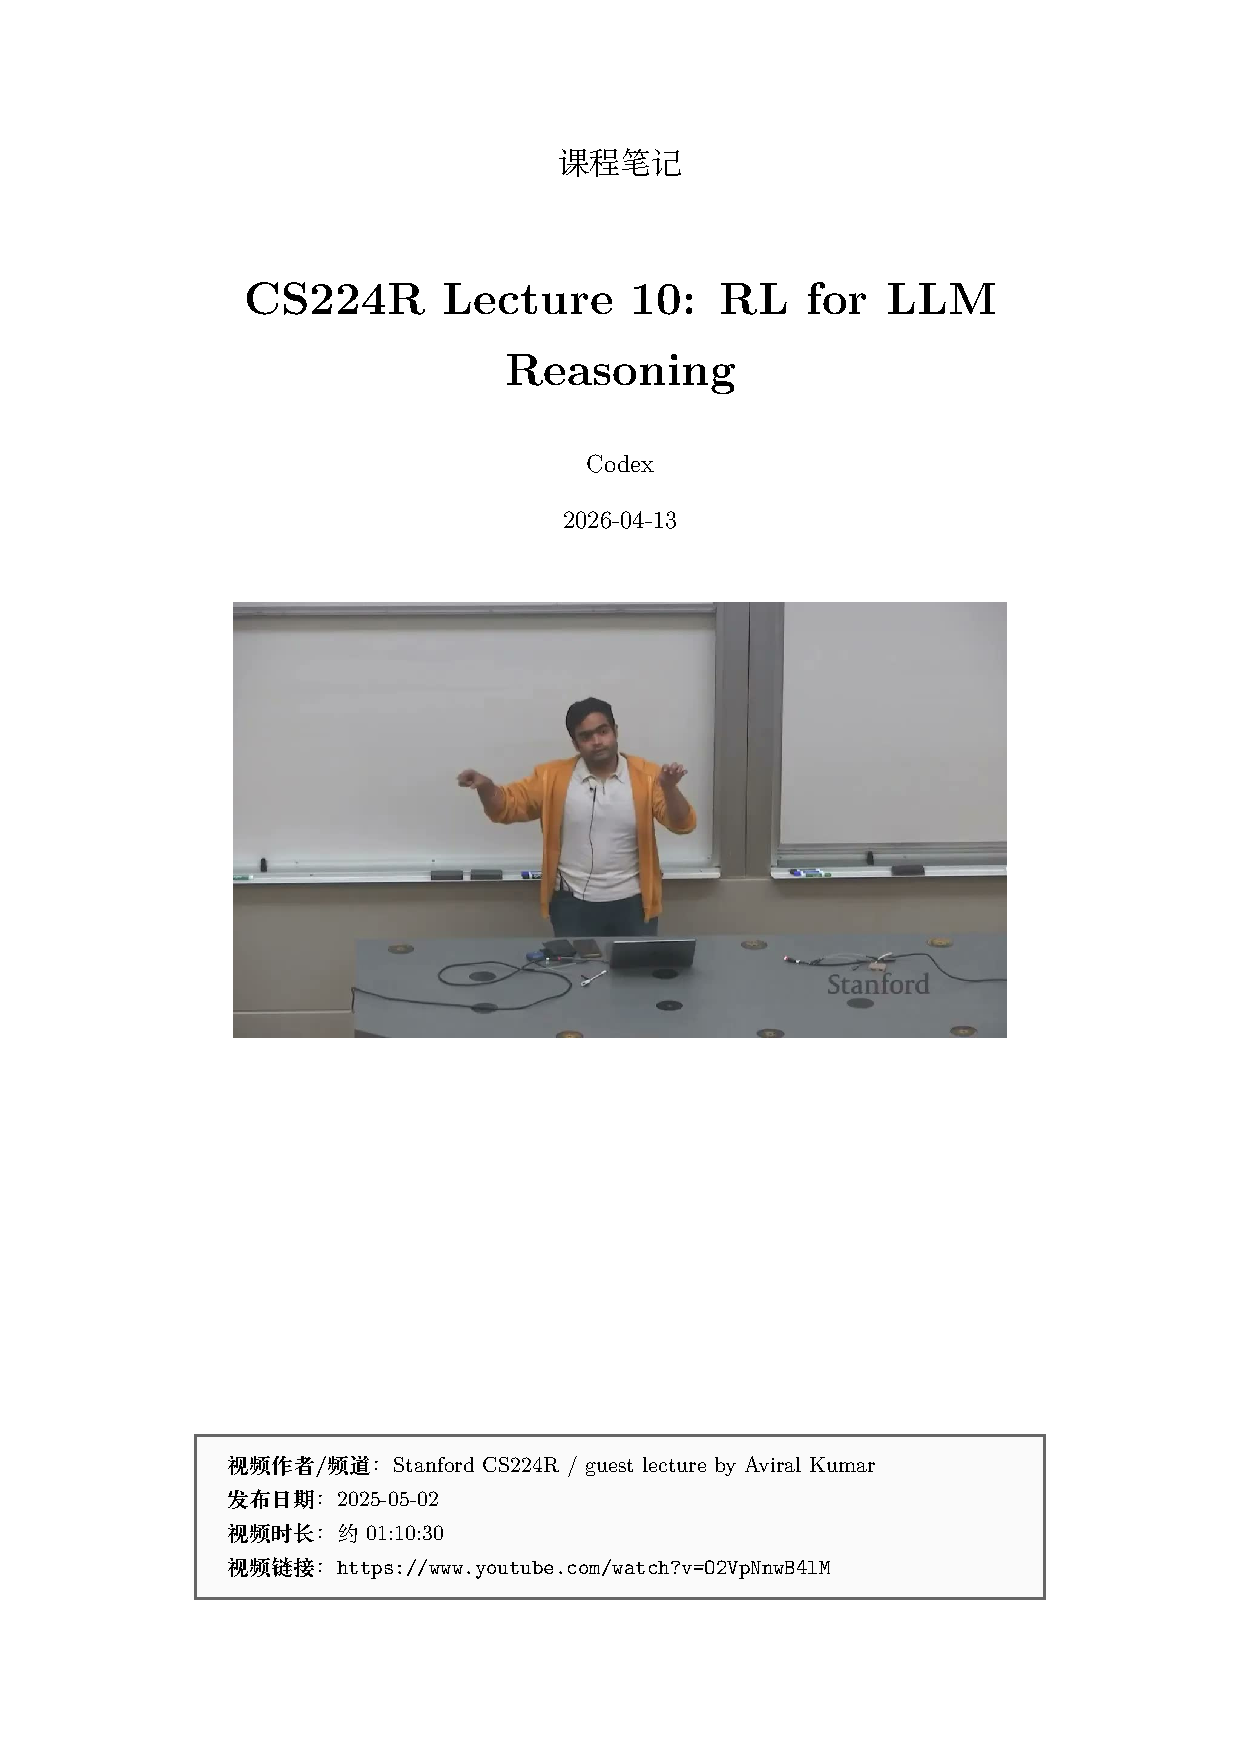
\includepdf[pages=-,pagecommand={\thispagestyle{plain}}]{../lectures/10_rl_for_llm_reasoning/lecture_10_note.pdf}

\section{Lecture 11: Model-Based RL}
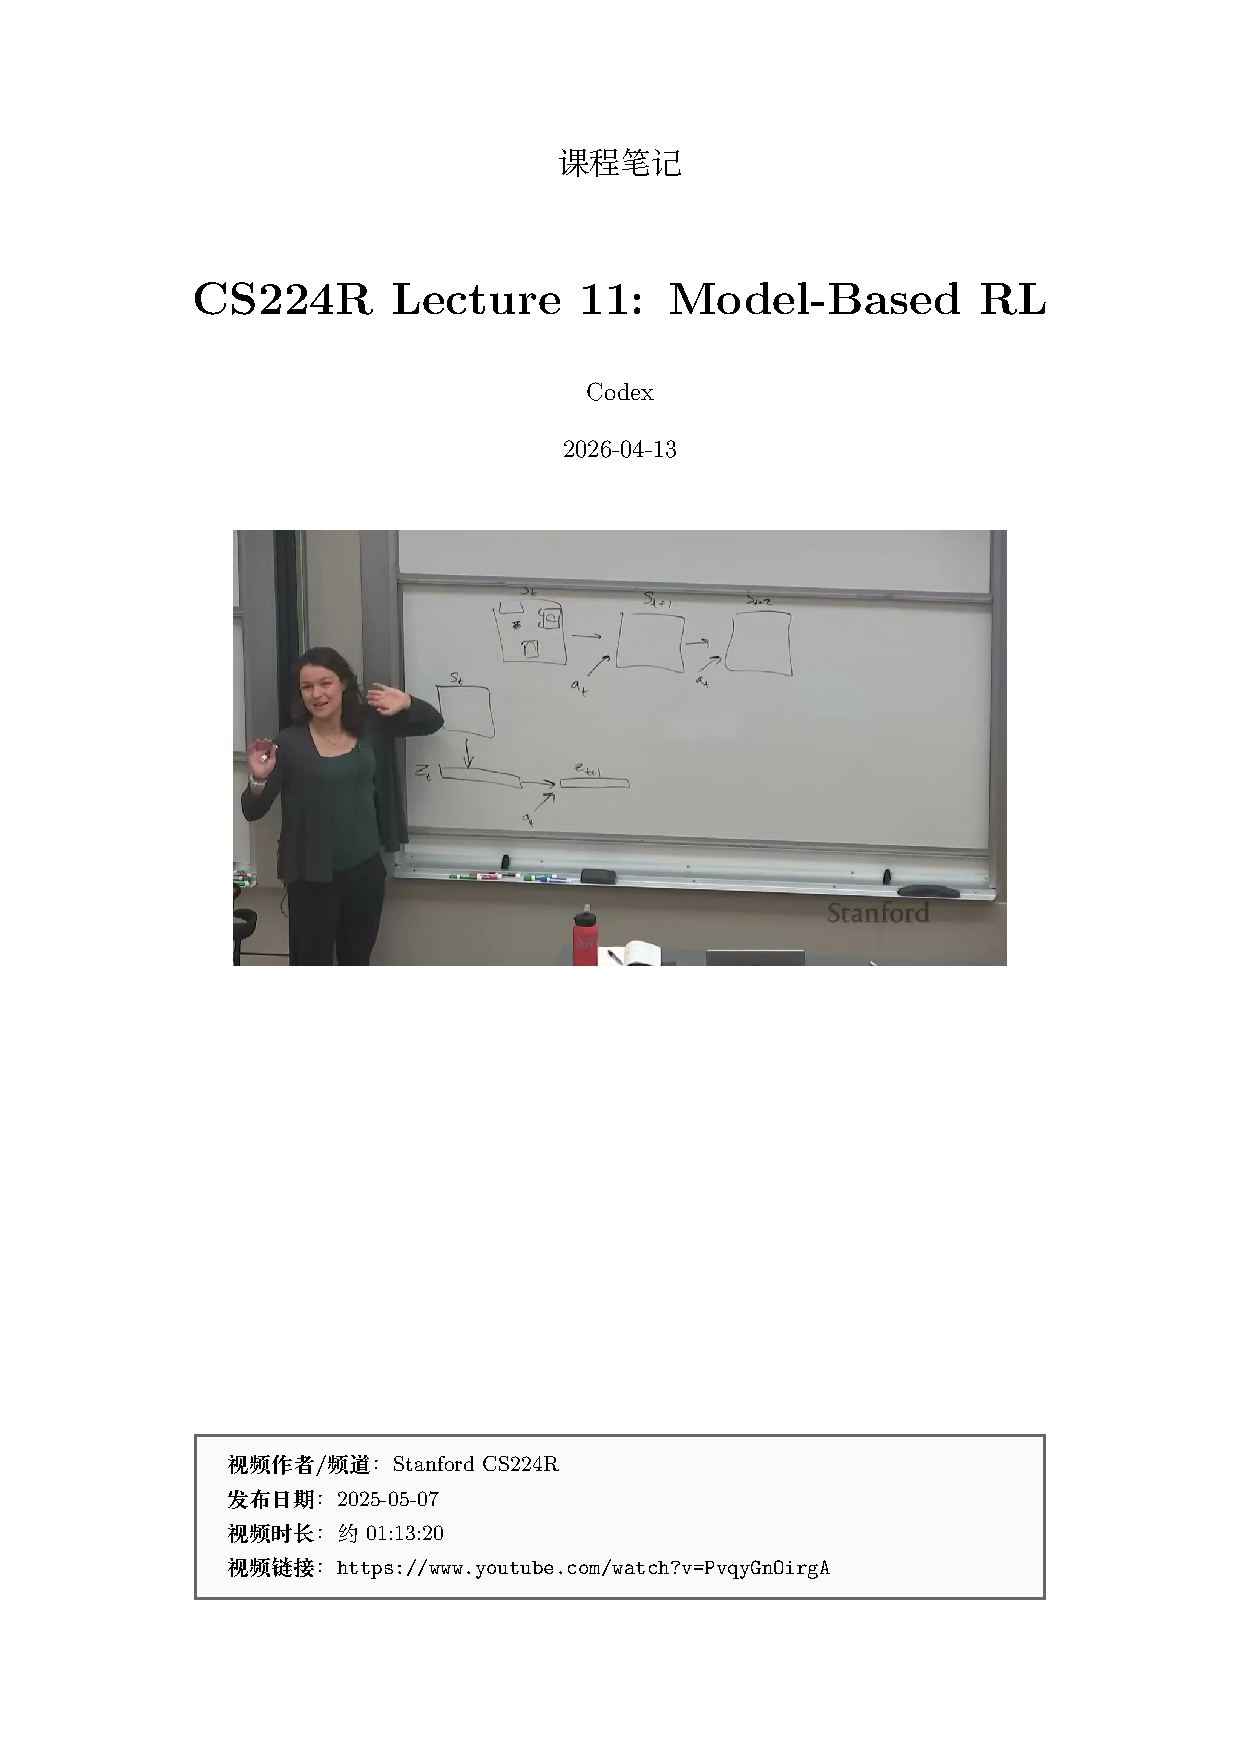
\includepdf[pages=-,pagecommand={\thispagestyle{plain}}]{../lectures/11_model_based_rl/lecture_11_note.pdf}

\section{Lecture 12: Multi-Task RL}
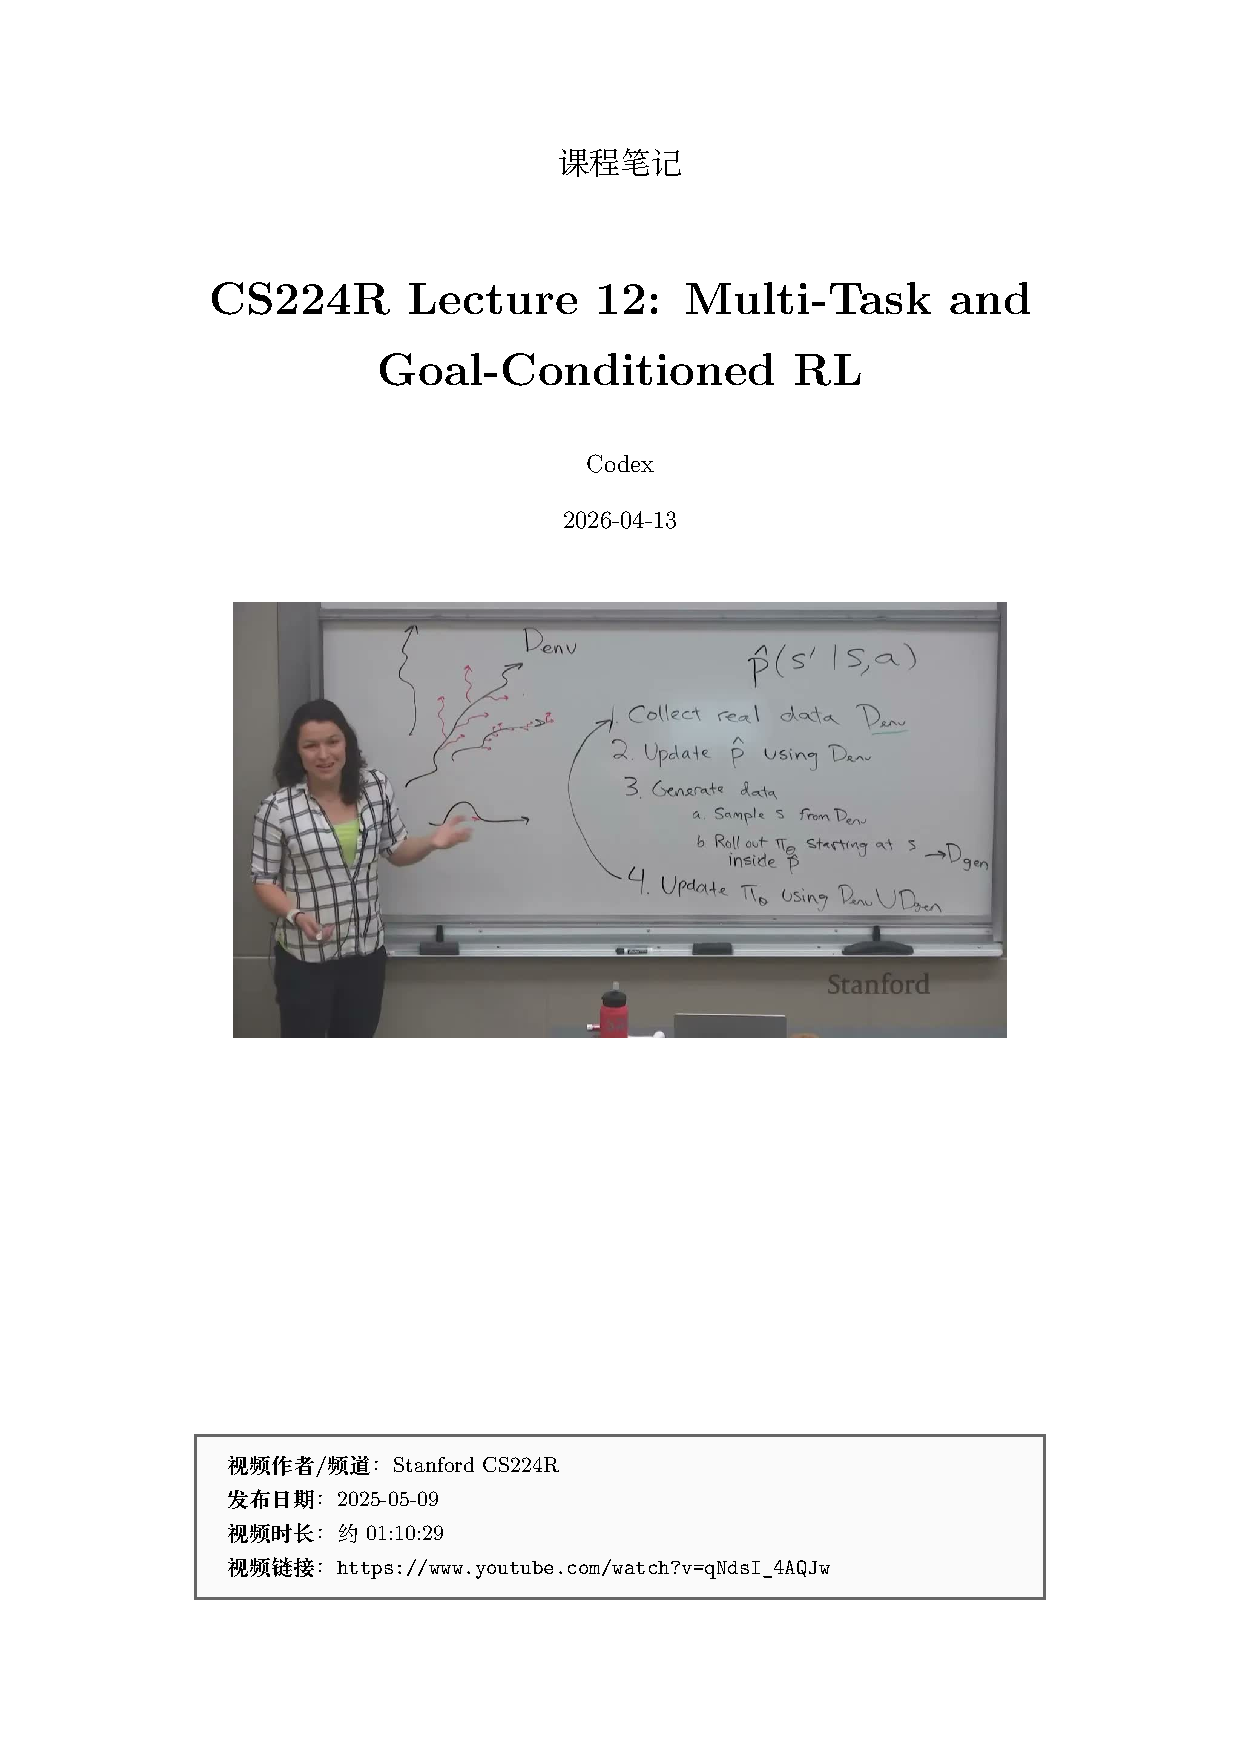
\includepdf[pages=-,pagecommand={\thispagestyle{plain}}]{../lectures/12_multi_task_rl/lecture_12_note.pdf}

\section{Lecture 13: Meta RL}
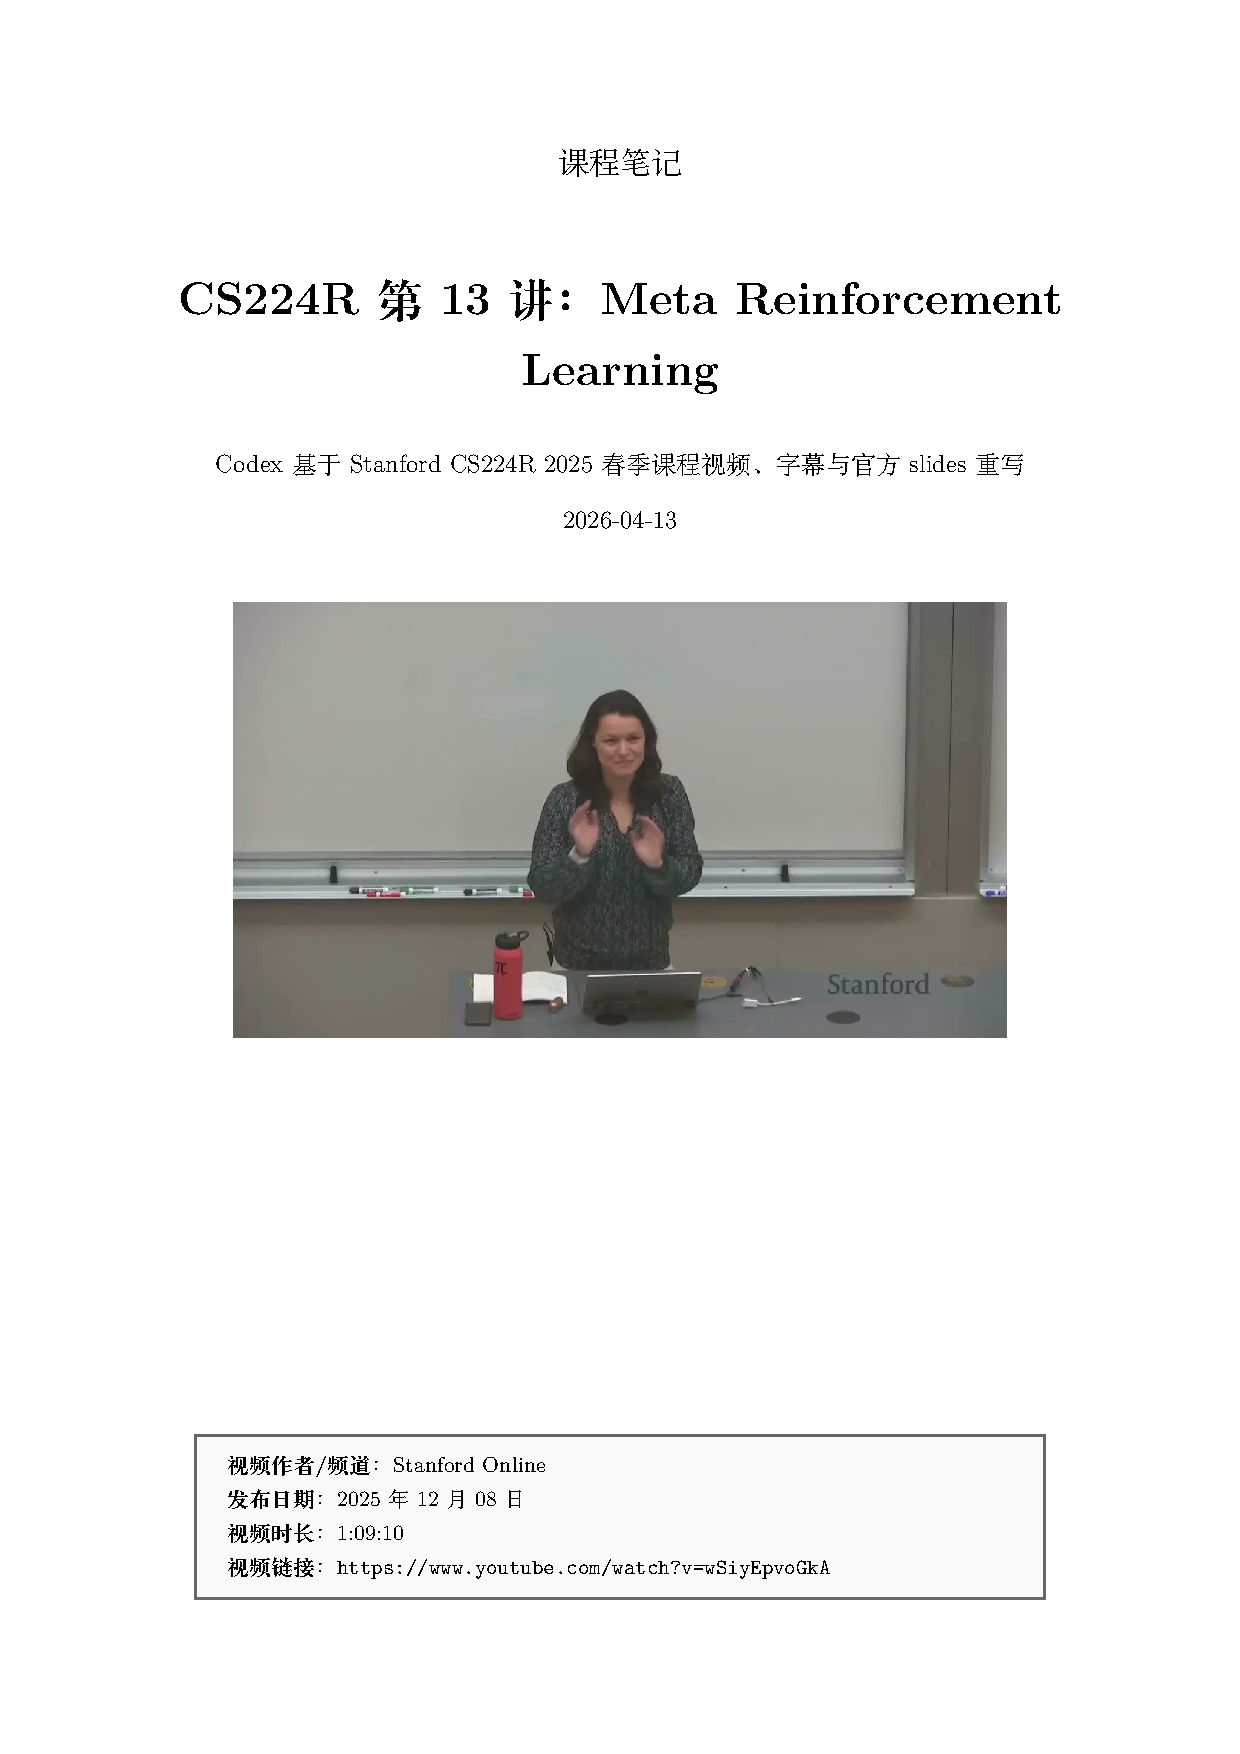
\includepdf[pages=-,pagecommand={\thispagestyle{plain}}]{../lectures/13_meta_rl/lecture_13_note.pdf}

\section{Lecture 14: Exploration}
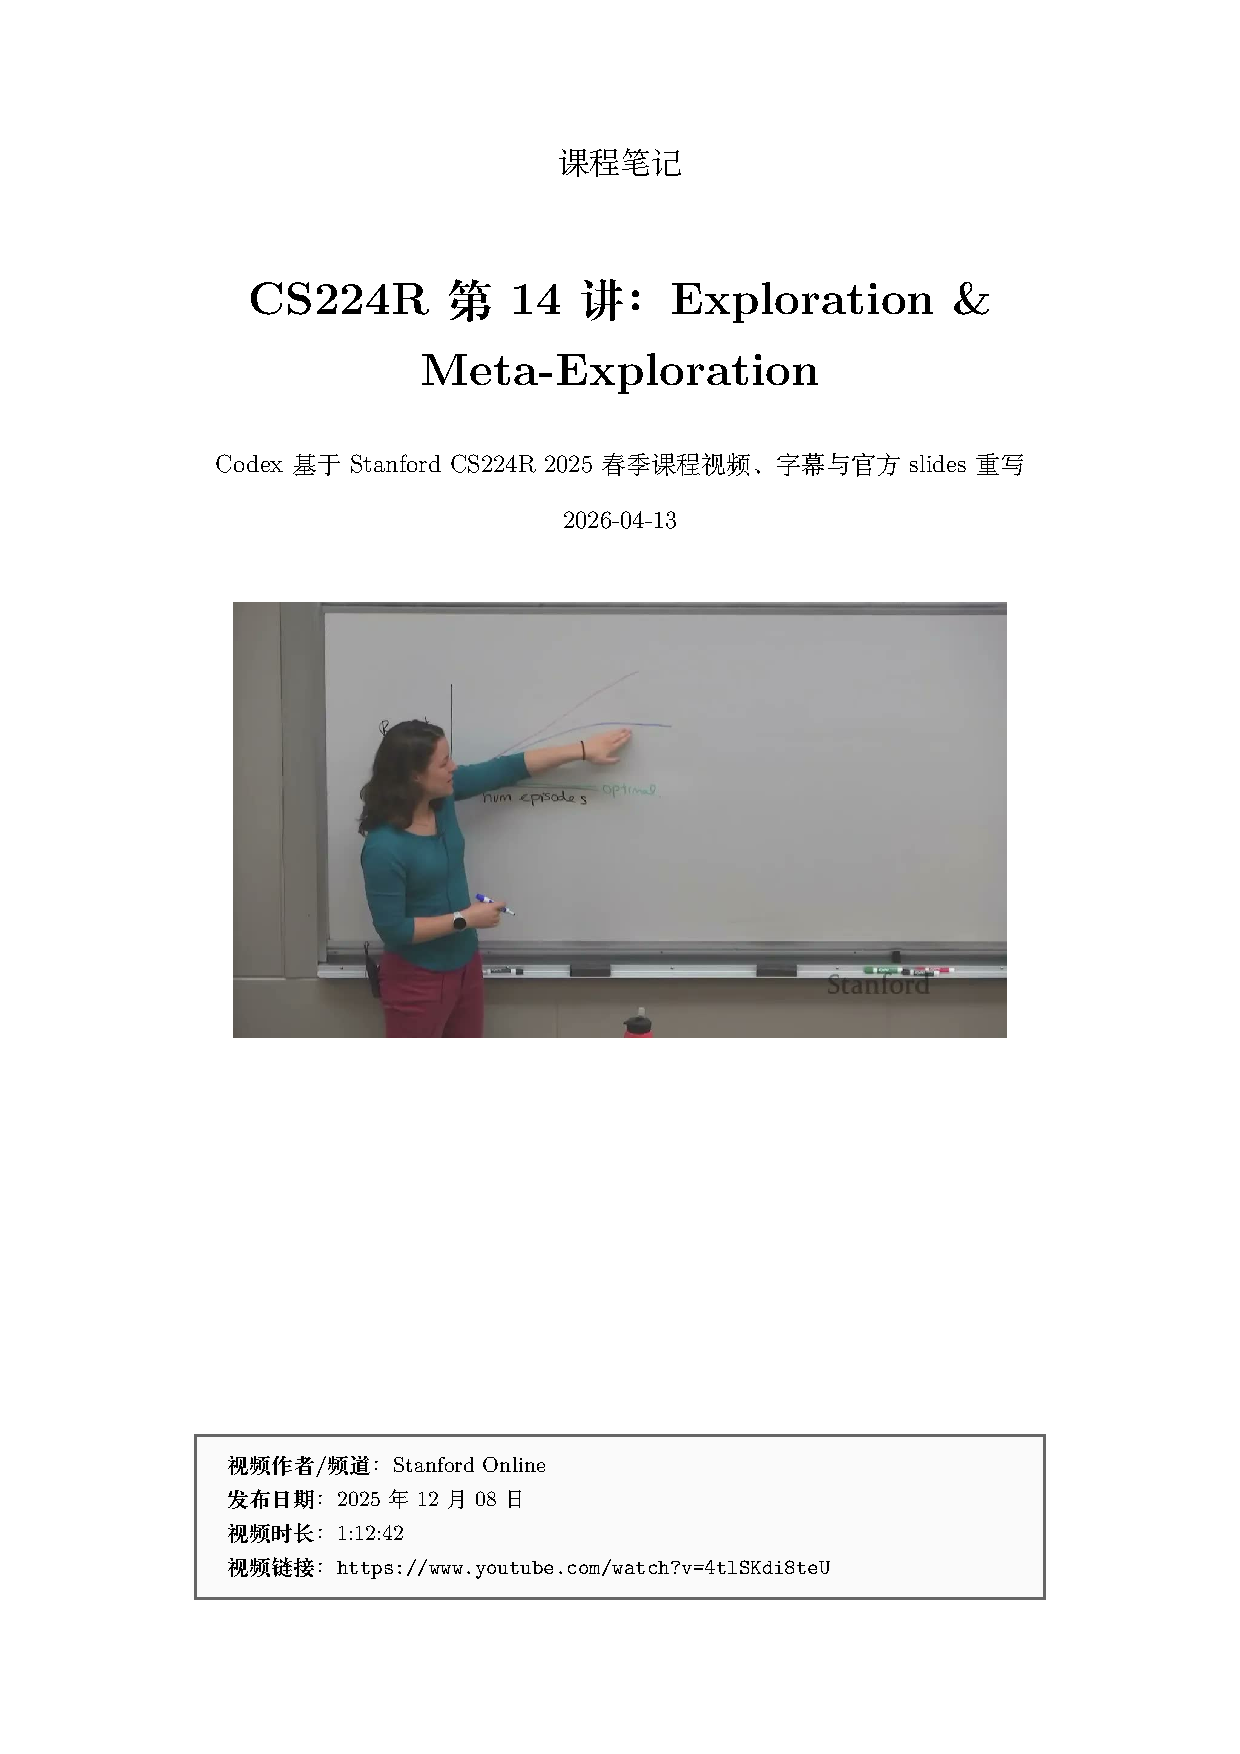
\includepdf[pages=-,pagecommand={\thispagestyle{plain}}]{../lectures/14_exploration/lecture_14_note.pdf}

\section{Lecture 15: Hierarchical RL and IL}
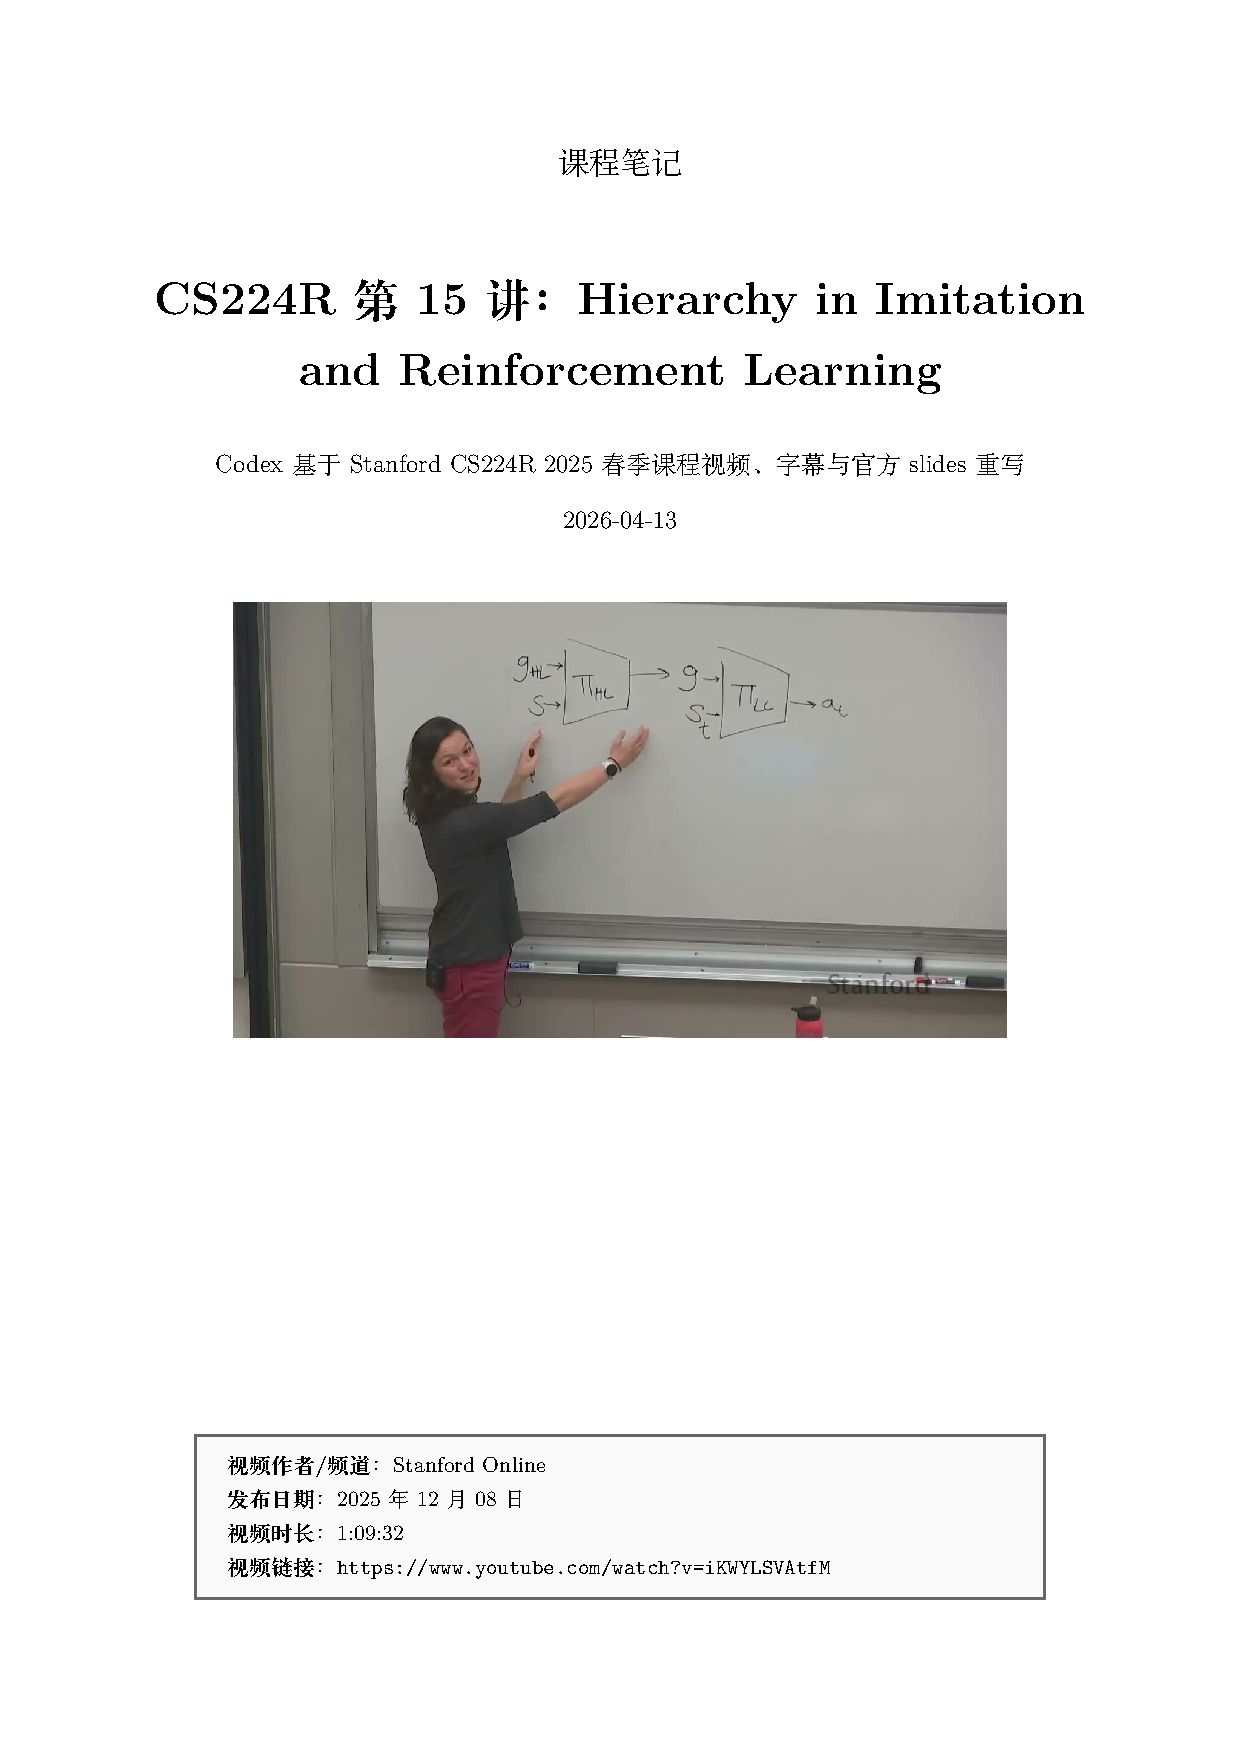
\includepdf[pages=-,pagecommand={\thispagestyle{plain}}]{../lectures/15_hierarchical_rl_and_il/lecture_15_note.pdf}

\section{Lecture 16: RL for Robots}
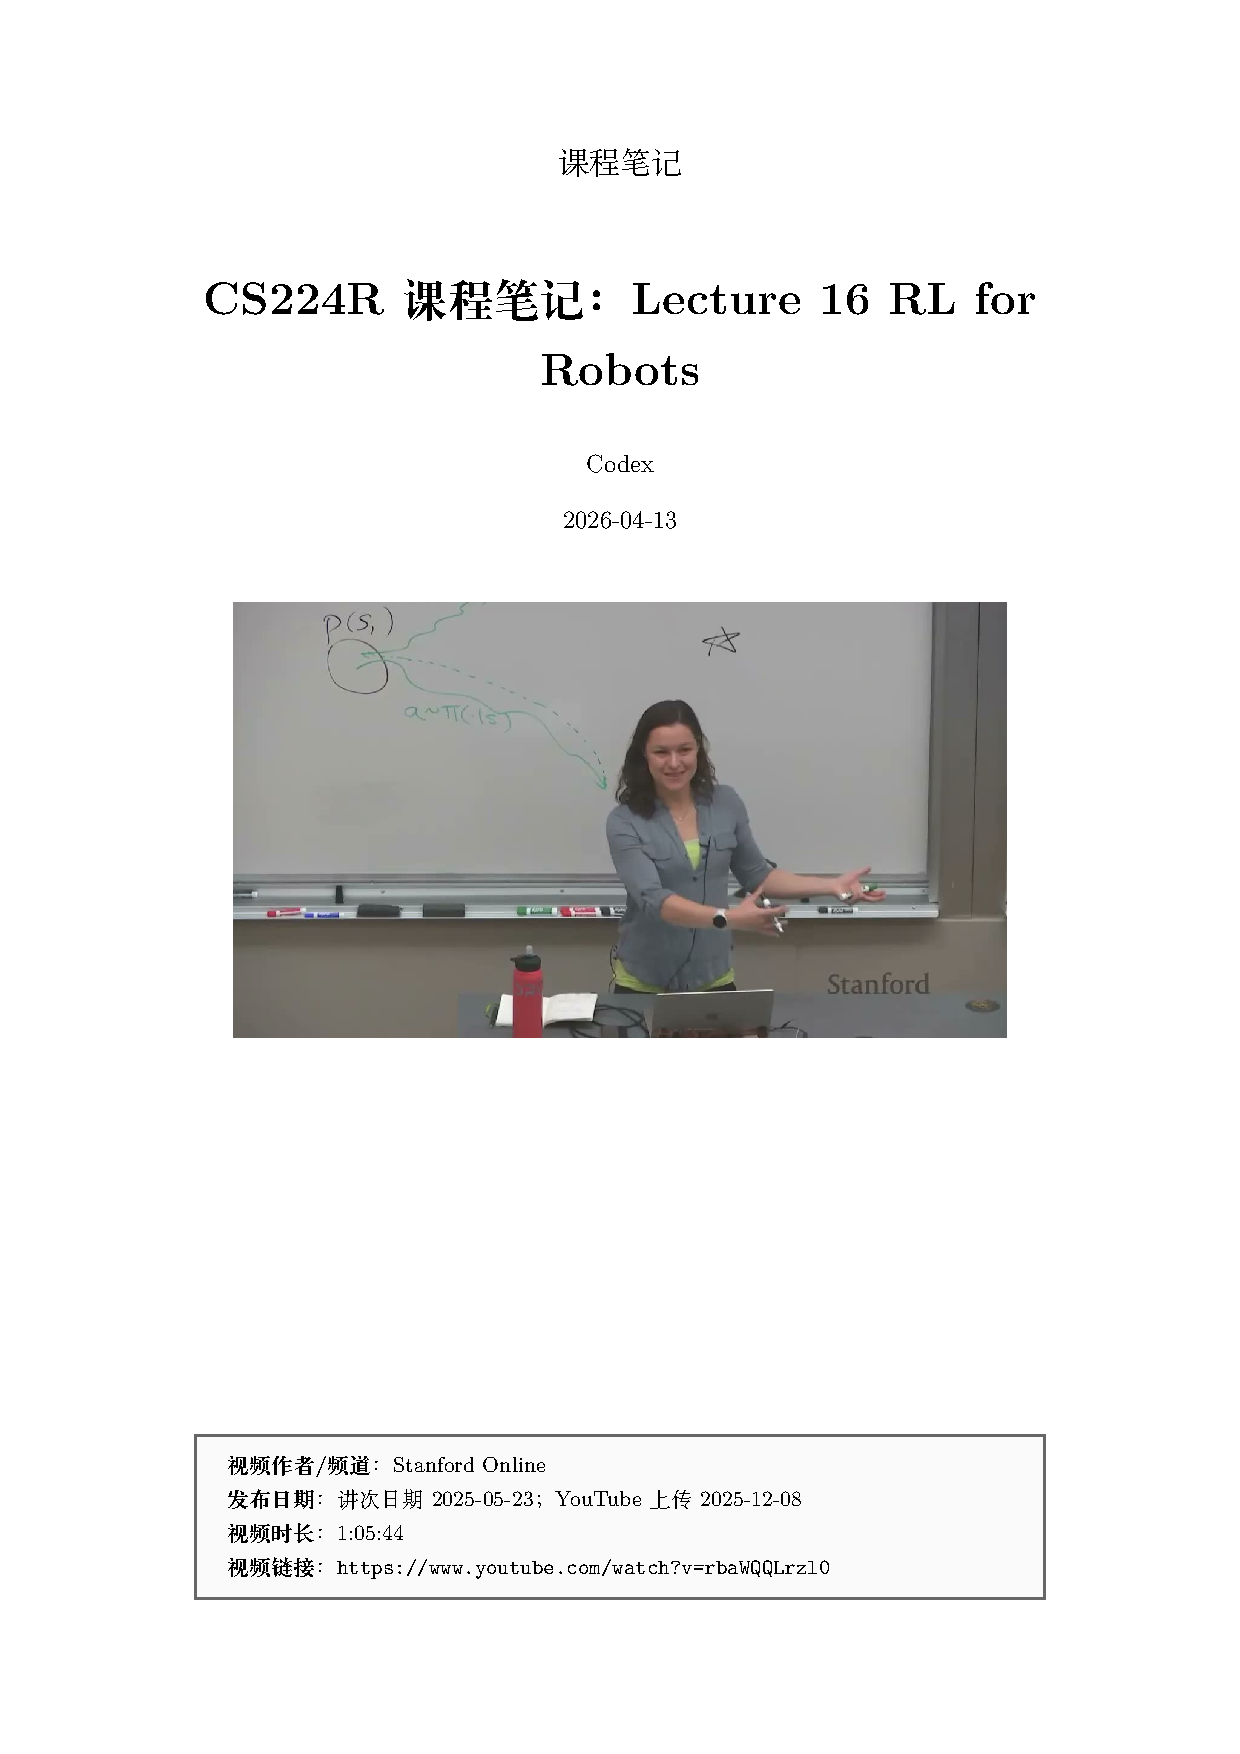
\includepdf[pages=-,pagecommand={\thispagestyle{plain}}]{../lectures/16_rl_for_robots/lecture_16_note.pdf}

\section{Lecture 17: Advancing Robot Intelligence}

\includepdf[pages=-,pagecommand={\thispagestyle{plain}}]{../lectures/17_advancing_robot_intelligence/lecture_17_note.pdf}

\section{Lecture 18: Frontiers}
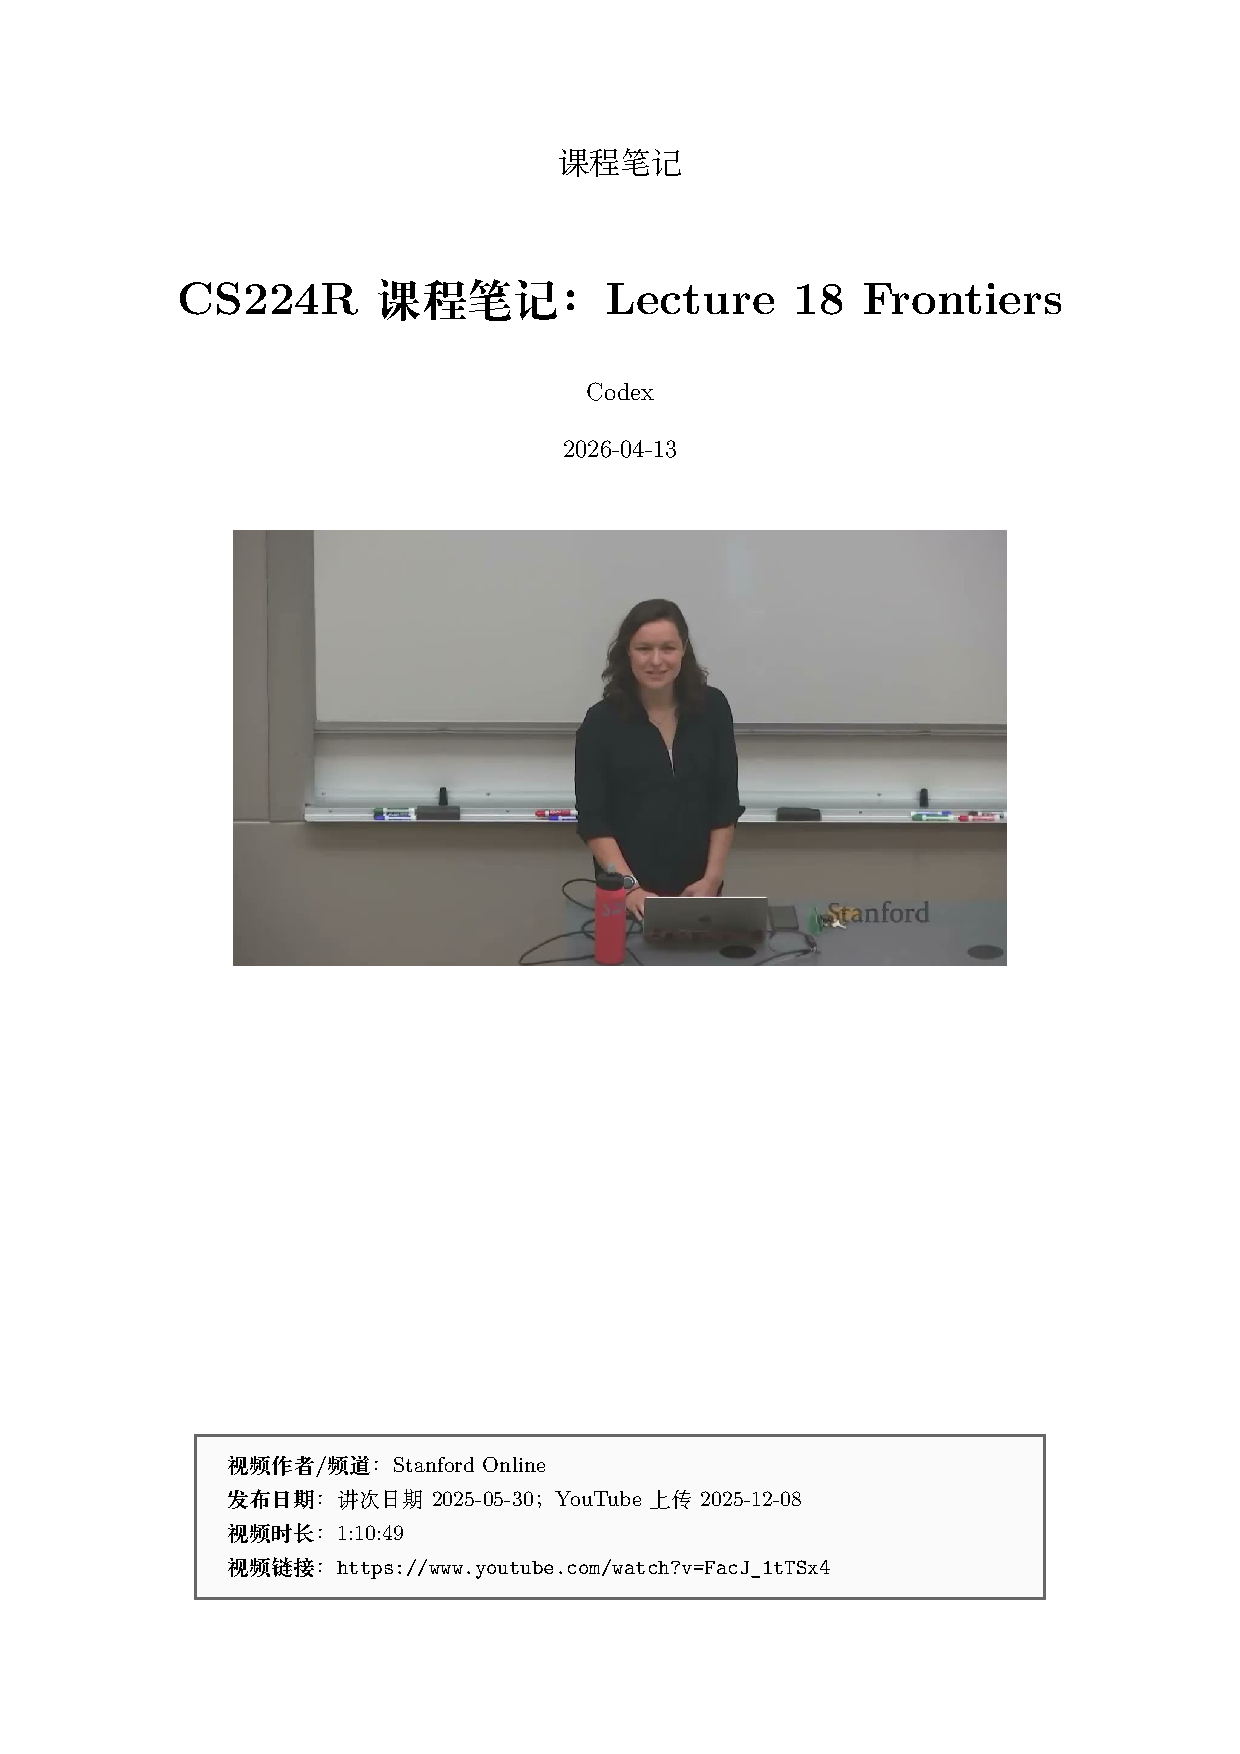
\includepdf[pages=-,pagecommand={\thispagestyle{plain}}]{../lectures/18_frontiers/lecture_18_note.pdf}

\section{Tutorial Session: Review of Q-Learning}
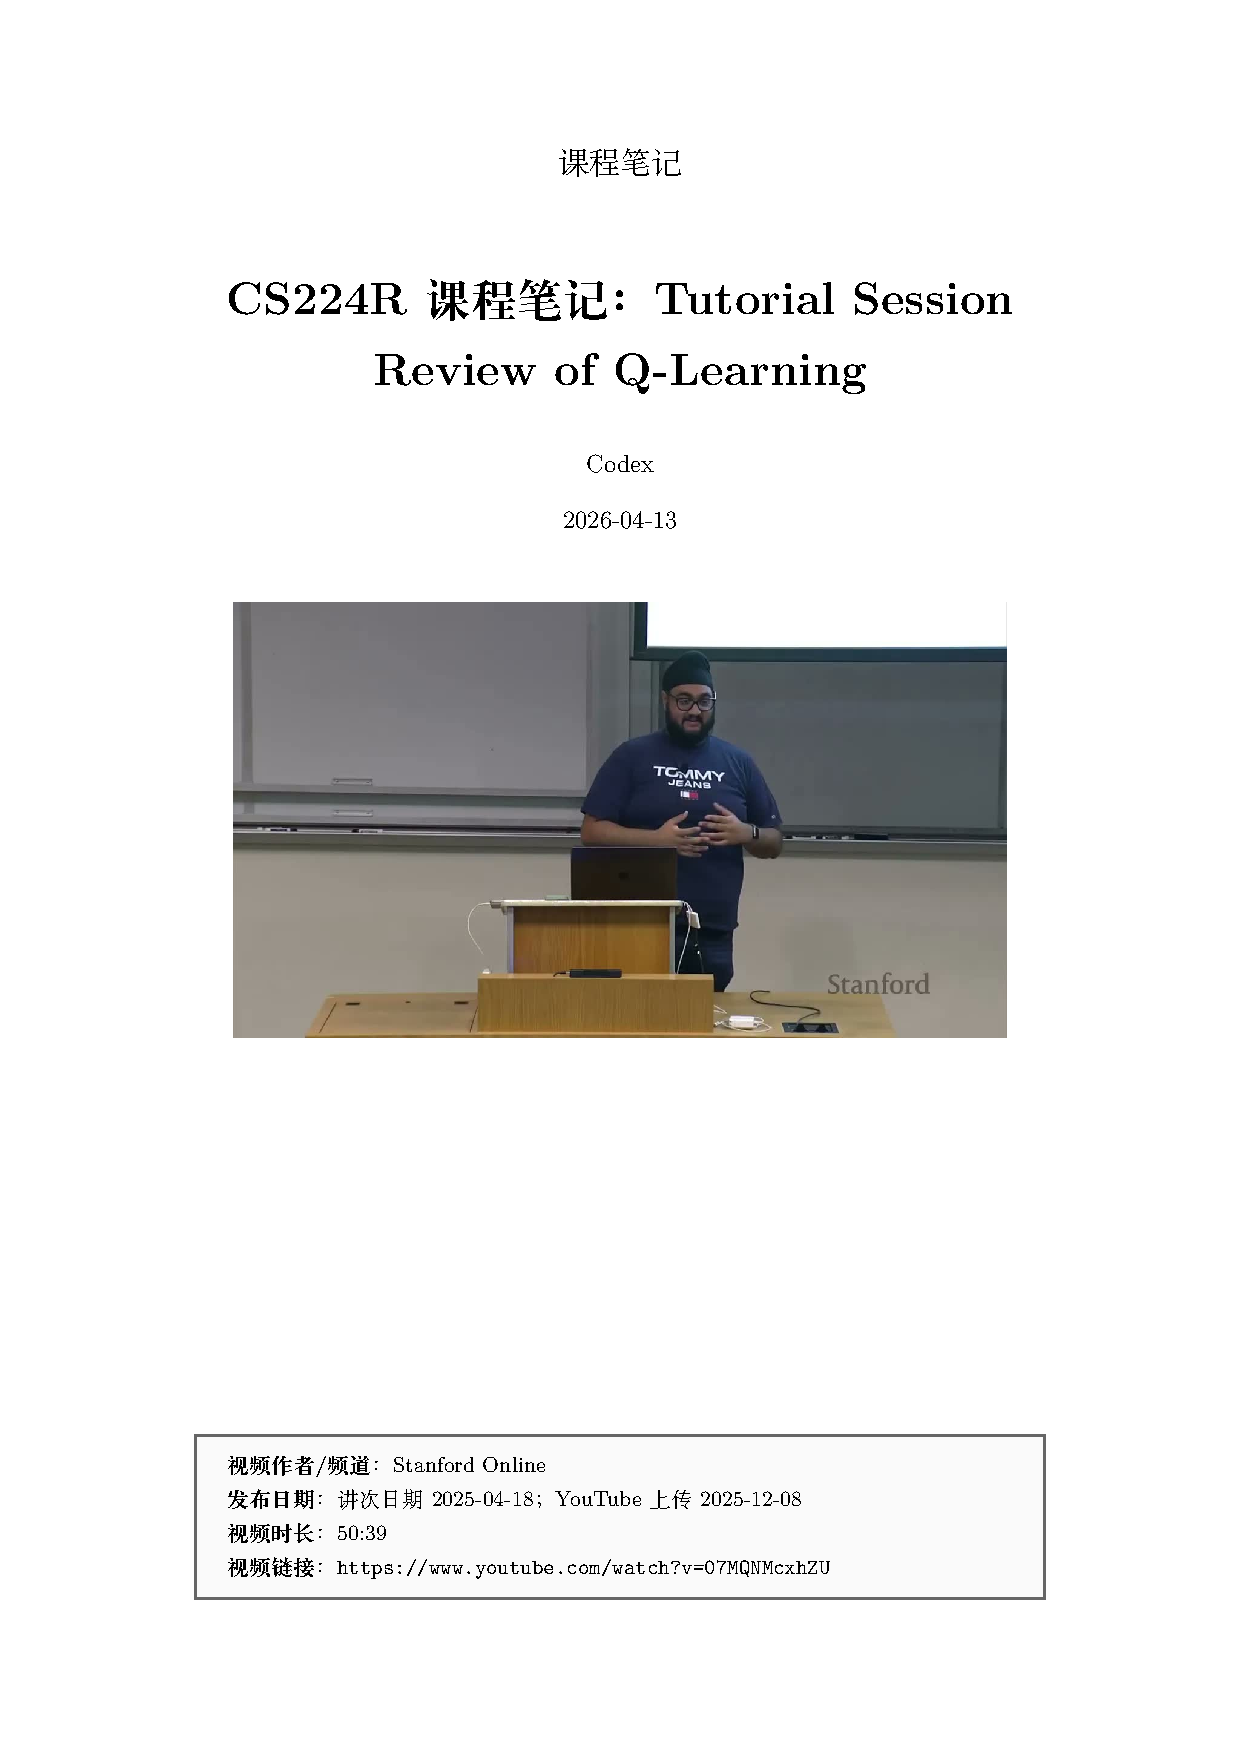
\includepdf[pages=-,pagecommand={\thispagestyle{plain}}]{../lectures/19_q_learning_tutorial/lecture_19_note.pdf}

\end{document}
